\documentclass{standalone}
\usepackage{tikz}
\usetikzlibrary{patterns, positioning}
\usepackage[sfdefault]{ClearSans} %% option 'sfdefault' activates Clear Sans as the default text font
\usepackage[T1]{fontenc}

\begin{document}
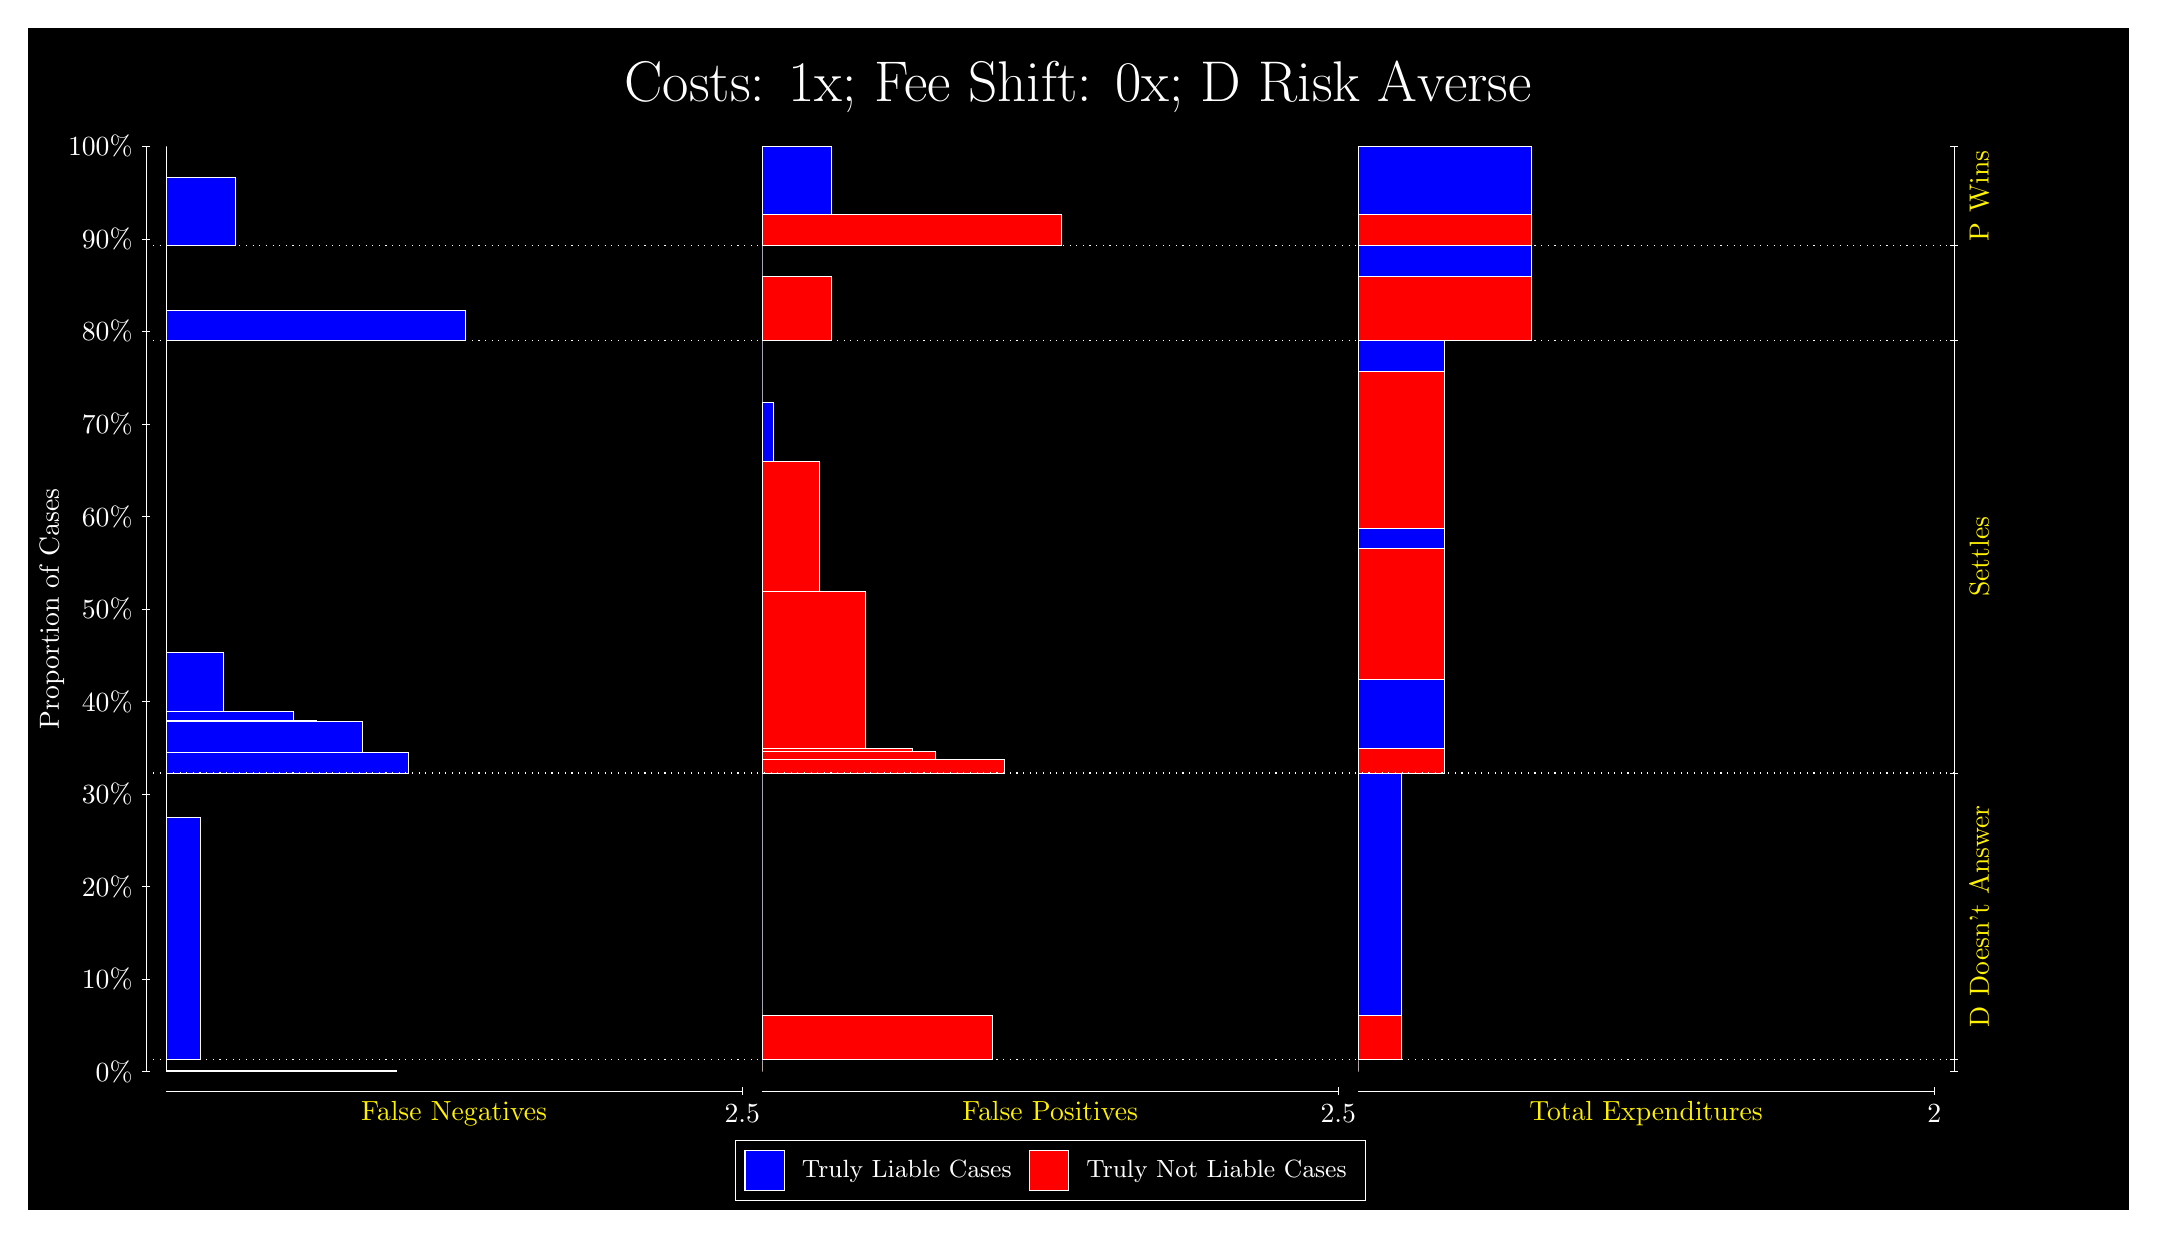
\begin{tikzpicture}
\draw[fill=black] (0,0) rectangle (26.667,15);
\draw[text=white] (0,13.5) rectangle (26.667,15) node[midway] {\huge Costs: 1x; Fee Shift: 0x; D Risk Averse};
\draw[white, very thin] (1.5,1.75) -- (1.5,13.5);
\node[rotate=90, text=white, anchor=center] at (0.3, 7.625) {Proportion of Cases};
\draw[white, very thin] (1.45,1.75) -- (1.55,1.75);
\node[text=white, anchor=east] at (1.45, 1.75) {0\%};
\draw[white, very thin] (1.45,2.925) -- (1.55,2.925);
\node[text=white, anchor=east] at (1.45, 2.925) {10\%};
\draw[white, very thin] (1.45,4.1) -- (1.55,4.1);
\node[text=white, anchor=east] at (1.45, 4.1) {20\%};
\draw[white, very thin] (1.45,5.275) -- (1.55,5.275);
\node[text=white, anchor=east] at (1.45, 5.275) {30\%};
\draw[white, very thin] (1.45,6.45) -- (1.55,6.45);
\node[text=white, anchor=east] at (1.45, 6.45) {40\%};
\draw[white, very thin] (1.45,7.625) -- (1.55,7.625);
\node[text=white, anchor=east] at (1.45, 7.625) {50\%};
\draw[white, very thin] (1.45,8.8) -- (1.55,8.8);
\node[text=white, anchor=east] at (1.45, 8.8) {60\%};
\draw[white, very thin] (1.45,9.975) -- (1.55,9.975);
\node[text=white, anchor=east] at (1.45, 9.975) {70\%};
\draw[white, very thin] (1.45,11.15) -- (1.55,11.15);
\node[text=white, anchor=east] at (1.45, 11.15) {80\%};
\draw[white, very thin] (1.45,12.325) -- (1.55,12.325);
\node[text=white, anchor=east] at (1.45, 12.325) {90\%};
\draw[white, very thin] (1.45,13.5) -- (1.55,13.5);
\node[text=white, anchor=east] at (1.45, 13.5) {100\%};

\draw[white, very thin] (24.457,1.75) -- (24.457,13.5);
\draw[white, very thin] (24.407,1.75) -- (24.507,1.75);
\node[anchor=west] at (24.407, 1.75) {};
\draw[white, very thin] (24.407,1.9053) -- (24.507,1.9053);
\node[anchor=west] at (24.407, 1.9053) {};
\draw[white, very thin] (24.407,5.5417) -- (24.507,5.5417);
\node[anchor=west] at (24.407, 5.5417) {};
\draw[white, very thin] (24.407,11.034) -- (24.507,11.034);
\node[anchor=west] at (24.407, 11.034) {};
\draw[white, very thin] (24.407,12.245) -- (24.507,12.245);
\node[anchor=west] at (24.407, 12.245) {};
\draw[white, very thin] (24.407,13.5) -- (24.507,13.5);
\node[anchor=west] at (24.407, 13.5) {};

\draw[white, very thin, fill=blue] (1.75,1.75) rectangle (4.6775,1.7663);
\draw[white, very thin, fill=red] (1.75,1.7663) rectangle (1.75,1.9053);
\draw[white, very thin, fill=blue] (1.75,1.9053) rectangle (2.1891,4.9802);
\draw[white, very thin, fill=red] (1.75,4.9802) rectangle (1.75,5.5417);
\draw[white, very thin, fill=blue] (1.75,5.5417) rectangle (4.8239,5.8059);
\draw[white, very thin, fill=blue] (1.75,5.8059) rectangle (4.2384,6.1923);
\draw[white, very thin, fill=blue] (1.75,6.1923) rectangle (3.6529,6.2069);
\draw[white, very thin, fill=blue] (1.75,6.2069) rectangle (3.3602,6.3243);
\draw[white, very thin, fill=blue] (1.75,6.3243) rectangle (2.4819,7.0703);
\draw[white, very thin, fill=red] (1.75,7.0703) rectangle (1.75,11.034);
\draw[white, very thin, fill=blue] (1.75,11.034) rectangle (5.5558,11.423);
\draw[white, very thin, fill=red] (1.75,11.423) rectangle (1.75,12.245);
\draw[white, very thin, fill=blue] (1.75,12.245) rectangle (2.6283,13.11);
\draw[white, very thin, fill=red] (1.75,13.11) rectangle (1.75,13.5);
\draw[white, very thin, fill=red] (9.3189,1.75) rectangle (9.3189,1.889);
\draw[white, very thin, fill=blue] (9.3189,1.889) rectangle (9.3189,1.9053);
\draw[white, very thin, fill=red] (9.3189,1.9053) rectangle (12.246,2.4669);
\draw[white, very thin, fill=blue] (9.3189,2.4669) rectangle (9.3189,5.5417);
\draw[white, very thin, fill=red] (9.3189,5.5417) rectangle (12.393,5.7163);
\draw[white, very thin, fill=red] (9.3189,5.7163) rectangle (11.515,5.8178);
\draw[white, very thin, fill=red] (9.3189,5.8178) rectangle (11.222,5.8587);
\draw[white, very thin, fill=red] (9.3189,5.8587) rectangle (10.636,7.8524);
\draw[white, very thin, fill=red] (9.3189,7.8524) rectangle (10.051,9.5051);
\draw[white, very thin, fill=blue] (9.3189,9.5051) rectangle (9.4652,10.251);
\draw[white, very thin, fill=blue] (9.3189,10.251) rectangle (9.3189,11.034);
\draw[white, very thin, fill=red] (9.3189,11.034) rectangle (10.197,11.855);
\draw[white, very thin, fill=blue] (9.3189,11.855) rectangle (9.3189,12.245);
\draw[white, very thin, fill=red] (9.3189,12.245) rectangle (13.125,12.634);
\draw[white, very thin, fill=blue] (9.3189,12.634) rectangle (10.197,13.5);
\draw[white, very thin, fill=red] (16.888,1.75) rectangle (16.888,1.889);
\draw[white, very thin, fill=blue] (16.888,1.889) rectangle (16.888,1.9053);
\draw[white, very thin, fill=red] (16.888,1.9053) rectangle (17.437,2.4669);
\draw[white, very thin, fill=blue] (16.888,2.4669) rectangle (17.437,5.5417);
\draw[white, very thin, fill=red] (16.888,5.5417) rectangle (17.986,5.8587);
\draw[white, very thin, fill=blue] (16.888,5.8587) rectangle (17.986,6.7367);
\draw[white, very thin, fill=red] (16.888,6.7367) rectangle (17.986,8.3894);
\draw[white, very thin, fill=blue] (16.888,8.3894) rectangle (17.986,8.6536);
\draw[white, very thin, fill=red] (16.888,8.6536) rectangle (17.986,10.647);
\draw[white, very thin, fill=blue] (16.888,10.647) rectangle (17.986,11.034);
\draw[white, very thin, fill=red] (16.888,11.034) rectangle (19.083,11.855);
\draw[white, very thin, fill=blue] (16.888,11.855) rectangle (19.083,12.245);
\draw[white, very thin, fill=red] (16.888,12.245) rectangle (19.083,12.634);
\draw[white, very thin, fill=blue] (16.888,12.634) rectangle (19.083,13.5);
\draw[white, dotted] (1.5,1.9053) -- (24.457,1.9053);
\draw[white, dotted] (1.5,5.5417) -- (24.457,5.5417);
\draw[white, dotted] (1.5,11.034) -- (24.457,11.034);
\draw[white, dotted] (1.5,12.245) -- (24.457,12.245);
\draw[white, very thin] (1.75,1.5) -- (9.0689,1.5);
\node[text=yellow, anchor=north] at (5.4094, 1.5) {False Negatives};
\draw[white, very thin] (9.0689,1.45) -- (9.0689,1.55);
\node[text=white, anchor=north] at (9.0689, 1.45) {2.5};

\draw[white, very thin] (9.3189,1.5) -- (16.638,1.5);
\node[text=yellow, anchor=north] at (12.978, 1.5) {False Positives};
\draw[white, very thin] (16.638,1.45) -- (16.638,1.55);
\node[text=white, anchor=north] at (16.638, 1.45) {2.5};

\draw[white, very thin] (16.888,1.5) -- (24.207,1.5);
\node[text=yellow, anchor=north] at (20.547, 1.5) {Total Expenditures};
\draw[white, very thin] (24.207,1.45) -- (24.207,1.55);
\node[text=white, anchor=north] at (24.207, 1.45) {2};


\node[text=yellow, centered, rotate=90] at (24.777, 3.7235) {D Doesn't Answer};
\node[text=yellow, centered, rotate=90] at (24.777, 8.2877) {Settles};

\node[text=yellow, centered, rotate=90] at (24.777, 12.872) {P Wins};

\draw (12.978300999999998,1.5) node[draw=none] (baseCoordinate) {};
\begin{scope}[align=center]
        \matrix[scale=0.5, draw=white, below=0.5cm of baseCoordinate, nodes={draw}, column sep=0.1cm]{
            \node[rectangle, draw, minimum width=0.5cm, minimum height=0.5cm, fill=blue] {}; &
            \node[draw=none, font=\small, text=white] (B) {Truly Liable Cases}; &
            \node[rectangle, draw, minimum width=0.5cm, minimum height=0.5cm, fill=red] {}; &
            \node[draw=none, font=\small, text=white] (B) {Truly Not Liable Cases}; \\
            };
\end{scope}

\end{tikzpicture}
\end{document}